\chapter{Test of Means of Continuous Data}

This chapter covers hypothesis tests for the mean value of groups:

\begin{itemize}
  \item Comparison of one group with a fixed value.
  \item Comparison if two groups with respect to each other.
  \item Comparison of three or more groups with each other.
\end{itemize}

In each case we distinguish between two cases. If the data are approximately normally distributed, so called Parametric Tests can be used\index{general}{parameteric test}. These tests are more sensitive than "non-parametric tests", but require that certain assumptions are fulfilled. If the data are not normally distributed, or if they are only available in ranked form, the corresponding non-parametric tests are presented\index{general}{non-parametric tests}.

\section{Distribution of a Sample Mean}

\subsection{One sample t-test for a mean value} \index{general}{test! t-test, one sample}

To check the mean value of normally distributed data against a reference value, we typically use the \emph{one sample t-test}, which is based on the t-distribution.

If we knew the mean and the standard deviation of a normally distributed population, we could calculate the corresponding standard error, and use values from the normal distribution to determine how likely it is to find a certain mean value, given the population mean and standard deviation. However, in practice we have to estimate the mean and standard deviation from the sample, and the t-distribution, which characterices the distribution of sample means for normally distributed data, deviates slightly from the normal distribution.

\subsubsection{Example}

Since it is very important to understand the basic principles of how to calculate the t-statistic and the corresponding p-value for this test, let me illustrate the underlying statistics by going through the analysis of a specific example, step-by-step. As example we take 100 normally distributed data, with a mean of 7 and with a standard deviation of 3.
What is the chance of finding a mean value at a distance of 0.5 or more from the mean? \emph{Answer: The probability from the t-test in the example is 0.057, and from the normal distribution 0.054.}


\begin{figure}
  \centering
  \includegraphics[width=0.75\textwidth]{../Images/ttestExplained.png}\\
  \caption{Left: Frequency histogram of the sample data, together with a normal fit. The sample mean, which is very close to the population mean, is indicated with a yellow triangle; the value to be checked with a red triangle. Right: sampling distribution of t (for n-1 degrees of freedom). At the bottom the normalized value of sample mean (yellow triangle) and value to be checked (red triangle). The red shaded area corresponds to the p-value.}\label{fig:ttestExplained}
\end{figure}

\begin{itemize}
  \item We have a population, with a mean value of 7 and a standard deviation of 3.
  \item From that population an observer takes 100 random samples. The sample mean of the example shown in Fig. \ref{fig:ttestExplained} is 7.10, close to but different from the real mean. The sample standard deviation is 3.12, and the standard error of the mean 0.312. This gives the observer an idea about the variability of the population.
  \item The observer knows that the distribution of the sample mean follows a t-distribution, and that the standard error of the mean (SEM) characterizes the width of that distribution.
  \item How likely it is that the real mean has a value of $x_0$ (e.g. 6.5, indicated by the red triangle in Fig. \ref{fig:ttestExplained}, left)? To find that out, this value has to be transformed, by subtracting the sample mean, and dividing by the standard error. (Fig. \ref{fig:ttestExplained}, right). This provides the \emph{t-statistic} for this test (-1.93).
  \item The corresponding p-value, which tells us how likely it is that the real mean has a value of 6.5 or more extreme relative to the sample mean, is given by the red shaded area under the curve-wings: \emph{2*CDF(t-statistic) = 0.057}, which means that the difference to 6.5 is just not significant. (The factor "2" comes from the fact that we have to check in both tails.)
\end{itemize}

In \emph{Python}, test statistic and p-value for the one sample t-test can be calculated with

\begin{lstlisting}
      t, pVal = stats.ttest_1samp(data, checkValue)
\end{lstlisting}

\PyImg "oneSample.py" (p \pageref{py:oneSample}): Sample analysis for one group of continuous data.
\index{python}{oneSample}

\subsection{Wilcoxon signed rank sum test}\index{general}{test!Wilcoxon signed rank sum}

If the data are not normally distributed, the one-sample t-test should not be used (although this test is fairly robust against deviations from normality, see Fig. \ref{fig:ttest_stability}). Instead, we must use a non-parametric test on the mean value. We can do this by performing a \emph{Wilcoxon signed rank sum test}. Note that in contrast to the one-sample t-test, this test checks for a difference from null:

\begin{lstlisting}
    (rank, pVal) = stats.wilcoxon(data-checkValue)
\end{lstlisting}

\footnote{The following description and example has been taken from \cite{altman99}, Table 9.2}
This method has three steps:

\begin{enumerate}
  \item Calculate the difference between each observation and the value of interest.
  \item Ignoring the signs of the differences, rank them in order of magnitude.
  \item Calculate the sum of the ranks of all the negative (or positive) ranks, corresponding to the observations below (or above) the chosen hypothetical value.
\end{enumerate}

In Table \ref{tab:wilcoxon} you see an example, where the significance to a deviation from the value of 7725 is tested. The rank sum of the negative values gives $3+5=8$, and can be looked up in the corresponding tables to be significant. In practice, your computer program will nowadays do this for you. This example also shows another feature of rank evaluations: tied values (here $7515$) get accorded their mean rank (here $1.5$).

\begin{table}
  \centering
  \begin{tabular}{l p{2.5cm} p{2.5cm} p{2.5cm}}
     \hline
     Subject & Daily energy intake (kJ) & Difference from 7725 kJ & Ranks of differences \\
     1 & 5260 & 2465 & 11 \\
     2 & 5470 & 2255 & 10 \\
     3 & 5640 & 2085 & 9 \\
     4 & 6180 & 1545 & 8 \\
     5 & 6390 & 1335 & 7 \\
     6 & 6515 & 1210 & 6 \\
     7 & 6805 & 920 & 4 \\
     8 & 7515 & 210 & 1.5 \\
     9 & 7515 & 210 & 1.5 \\
     10 & 8230 & -505 & 3 \\
     11 & 8770 & -1045 & 5 \\
     \hline
   \end{tabular}
  \caption{Daily energy intake of 11 healthy women with rank order of differences (ignoring their signs) from the recommended intake of 7725 kJ.}\label{tab:wilcoxon}
\end{table}


\section{Comparison of Two Groups} \index{general}{test! t-test, paired}

\subsection{Paired T-Test}
In the comparison of two groups with each other, two cases have to be distinguished. In the first case, two values recorded from the same subject at different times are compared to each other. For example, the size of students when they enter primary school and after their first year, to check if they have grown. Since we are only interested in the difference between the first and the second measurement, this test is called \gls{paired} t-test, and is essentially equivalent to a one-sample t-test for the mean difference.

Therefore the two tests \lstinline{stats.ttest_1samp} and \lstinline{stats.ttest_rel} provide the same result:

\begin{lstlisting}
  In [1]: import numpy as np
  In [2]: from scipy import stats

  In [3]: np.random.seed(1234)
  In [4]: data = np.random.randn(10)+0.1
  In [5]: data1 = np.random.randn(10)*5  # dummy data
  In [6]: data2 = data1 + data    # same difference between groups as "data"

  In [7]: stats.ttest_1samp(data, 0)
  Out[7]: (-0.12458492298731401, 0.90359045085470857)

  In [8]: stats.ttest_rel(data2, data1)
  Out[8]: (-0.1245849229873135, 0.9035904508547089)
\end{lstlisting}

\subsection{T-Test Between Independent Groups} \index{general}{test! t-test, independent groups}
An \gls{unpaired} t-test compares two independent groups. An example would be the comparison of the effect of a two medications given to two different groups of patients. This is called an \emph{unpaired t-test}, or \emph{t-test for two independent groups}.

If we have two independent samples the variance of the difference between their means is the sum of the separate variances, so the standard error of the difference in means is the square root of the sum of the separate variances:

\begin{align*}
   se({{\bar x}_1} \pm {{\bar x}_2}) &= \sqrt {\operatorname{var} ({{\bar x}_1}) + \operatorname{var} ({{\bar x}_2})}  \\
   &= \sqrt {{{\left\{ {se({{\bar x}_1})} \right\}}^2} + {{\left\{ {se({{\bar x}_2})} \right\}}^2}}  \\
   &= \sqrt {\frac{{s_1^2}}{{{n_1}}} + \frac{{s_2^2}}{{{n_2}}}}  \\
\end{align*}

where $\bar{x}_i$ is the mean of the i-th sample, and \emph{se} indicates the \emph{standard error}.

Expressed in words, \emph{The variance of a sum of independent random variables equals the sum of the variances.}

\begin{lstlisting}
    t_statistic, pVal = stats.ttest_ind(group1, group2)
\end{lstlisting}

\subsection{Non-parametric Comparison of Two Groups: Mann-Whitney Test} \index{general}{test!Mann-Whitney}\label{test:Mann-Whitney}

If the measurement values from the two groups are not normally distributed we have to resort to a non-parametric test. The most common test for that is the \emph{Mann-Whitney(-Wilcoxon) test}. Watch out, because this test is sometimes also referred to as \emph{Wilcoxon rank-sum test}. This is different from the \emph{Wilcoxon signed rank sum test}!
The test-statistic for this test is commonly indicated with \emph{u}:

\begin{lstlisting}
    u_statistic, pVal = stats.mannwhitneyu(group1, group2)
\end{lstlisting}


\PyImg "twoSample.py" (p \pageref{py:twoSample}): Comparison of two groups, paired and unpaired.
\index{python}{twoSample}

\subsection{Statistical Hypothesis Tests vs Statistical Modeling}

With the advent of cheap computing power, statistical modeling has been a booming field. This has also affected classical statistical analysis, as most problems can be viewed from two perspectives: one can either make a statistical hypothesis, and verify or falsify that hypothesis; or one can make a statistical model, and analyse the significance of the model parameters.

Let me use a classical t-test as an example.

\subsubsection{Classical t-test}

Let us take performance measurements from a racing team, on two different occasions. During Race\_1, the members of the team achieve a score of [ 79, 100, 93, 75, 84, 107, 66, 86, 103, 81, 83, 89, 105, 84, 86, 86, 112, 112, 100, 94], and during Race\_2 [ 92, 100, 76, 97, 72, 79, 94, 71, 84, 76, 82, 57, 67, 78, 94, 83, 85, 92, 76, 88].

These numbers can be generated, and a t-test comparing the two groups can be done, with the following \emph{Python} commands:

\begin{lstlisting}
    import numpy as np
    from scipy import stats

    random.seed(123)
    race_1 = np.round(randn(20)*10+90)
    race_2 = np.round(randn(20)*10+85)
    (t, pVal) = stats.ttest_rel (race_1, race_2)
    print('The probability that the two distributions are equal is {0}'.format(pVal))
\end{lstlisting}

The command \lstinline{random.seed(123)} initializes the random number generator with the number $123$, which ensures that two consecutive runs of this code produce the same result, corresponding to the numbers given above.

\subsubsection{Statistical Modeling}

\begin{lstlisting}
    import pandas as pd
    import statsmodels.formula.api as sm

    np.random.seed(123)
    df = pd.DataFrame({'Race1': race_1, 'Race2':race_2})
    result = sm.ols(formula='I(Race2-Race1) ~ 1', data=df).fit()
    print(result.summary())
\end{lstlisting}

The important line is the last but one, which produces the $results$. Thereby the function \lstinline{sm.ols}  ("ols" for "ordinary least square") function from \emph{statsmodels} tests the model which describes the difference between the results of \emph{Race1} and those of \emph{Race2} with only an offset (also called Intercept in the language of modeling). In other words, the model has only one parameter, the \emph{Intercept}. The results below show that the probability that this intercept is only $0.033$: the difference is significant.

 \small\begin{lstlisting}

                             OLS Regression Results
==============================================================================
Dep. Variable:       I(Race2 - Race1)   R-squared:                       0.000
Model:                            OLS   Adj. R-squared:                  0.000
Method:                 Least Squares   F-statistic:                       nan
Date:                Sun, 08 Feb 2015   Prob (F-statistic):                nan
Time:                        18:48:06   Log-Likelihood:                -85.296
No. Observations:                  20   AIC:                             172.6
Df Residuals:                      19   BIC:                             173.6
Df Model:                           0
Covariance Type:            nonrobust
==============================================================================
                 coef    std err          t      P>|t|      [95.0% Conf. Int.]
------------------------------------------------------------------------------
Intercept     -9.1000      3.950     -2.304      0.033       -17.367    -0.833
==============================================================================
Omnibus:                        0.894   Durbin-Watson:                   2.009
Prob(Omnibus):                  0.639   Jarque-Bera (JB):                0.793
Skew:                           0.428   Prob(JB):                        0.673
Kurtosis:                       2.532   Cond. No.                         1.00
==============================================================================
\end{lstlisting}
\normalsize

The output is explained in more detail in the chapter \ref{chapter:Models}. The important point here is that the t- and p-value for the intercept are the same as with the classical t-test above.

\section{Comparison of More Groups}

\subsection{Analysis of Variance - ANOVA} \label{sec:anova} \index{general}{ANOVA} \index{general}{test!ANOVA}

The idea behind the \acrfull{anova} (ANOVA) is to divide the variance into the variance \emph{between} groups, and that \emph{within} groups, and see if those distributions match the null hypothesis that all groups come from the same distribution. The variables that distinguish the different groups are often called Factors or Treatments.

\begin{figure}
  \centering
  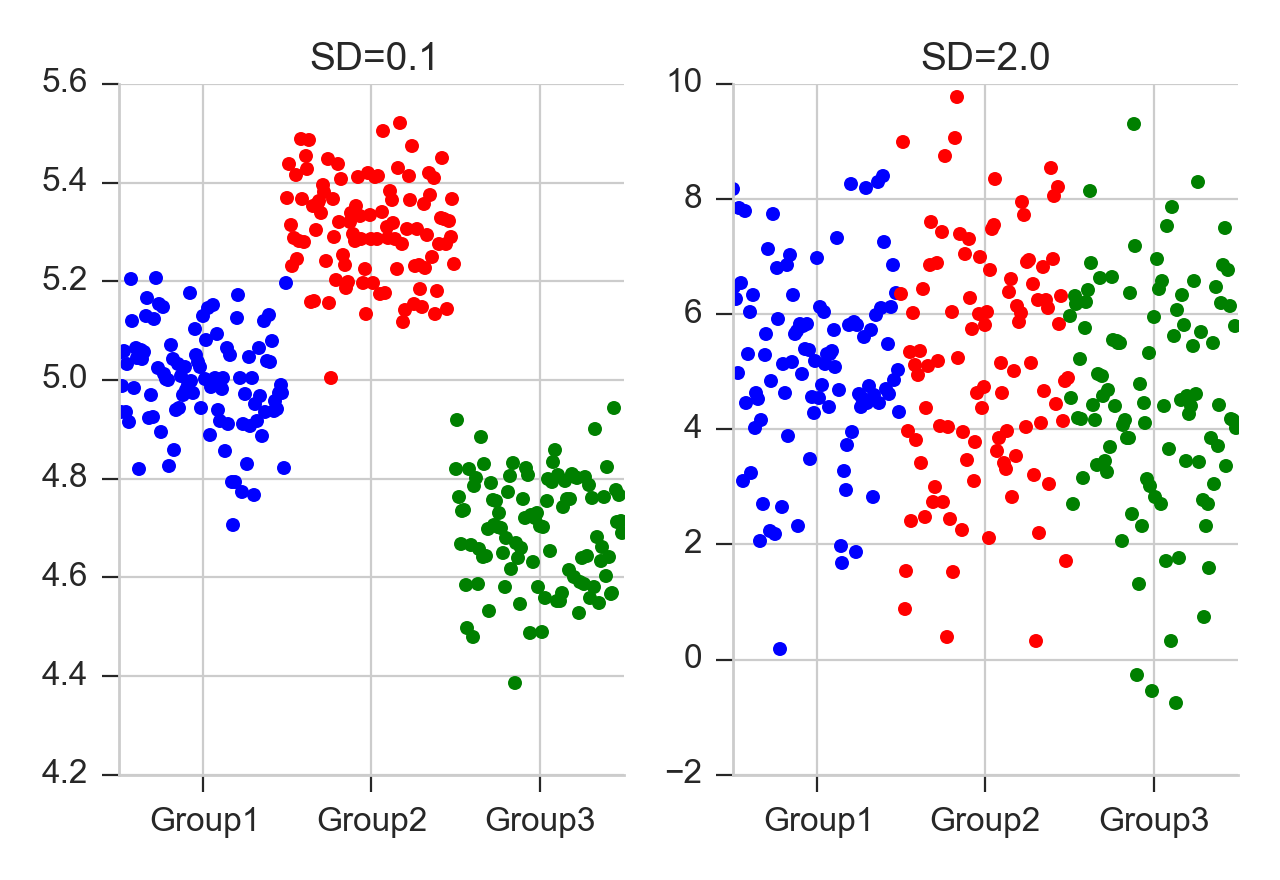
\includegraphics[width=0.75\textwidth]{../Images/ANOVA_oneway.png}\\
  \caption{In both cases, the difference between the two groups is the same. But left, he difference within the groups is smaller than the differences between the groups, whereas right, the difference within the groups is larger than the difference between.}\label{fig:ANOVA_oneway}
\end{figure}

(By comparison, t-tests look at the mean values of two groups, and check if those are consistent with the assumption that the two groups come from the same distribution.)

For example, if we compare a group with \emph{No treatment}, another with \emph{treatment A}, and a third with \emph{treatment B}, then we perform a "one factor ANOVA", sometimes also called "one-way ANOVA", with \emph{treatment} the one analysis factor. If we do the same test with men and with women, then we have a "two-factor" or "two-way ANOVA", with \emph{gender} and \emph{treatment} as the two treatment factors. Note that with ANOVAs, it is quite important to have exactly the same number of samples in each analysis group! (This is called a "balanced ANOVA"\index{general}{ANOVA!balanced}: a balanced design has an equal number of observations for all possible combinations of factor levels.)

Because the null hypothesis is that there is no difference between the groups, the test is based on a comparison of the observed variation between the groups (i.e. between their means) with that expected from the observed variability between subjects. The comparison takes the general form of an F-test to compare variances, but for two groups the t -test leads to exactly the same result.

The one-way ANOVA assumes all the samples are drawn from normally distributed populations with equal variance. To test the equal variance assumption, one of the popular approaches is the Levene test\index{general}{test!Levene}.

ANOVA uses traditional terminology. DF indicates the degrees of freedom (DF) (see also section \ref{sec:DF}), the summation is called the \acrfull{ss} (SS), the result is called the Mean Square (MS) and the squared terms are deviations from the sample mean.
In general, the sample variance\index{general}{sample variance} is defined by

\begin{equation}\label{eq:sampleVariance}
  s^2 = \frac{1}{DF} \sum (y_i - \bar{y})^2 = \frac{SS}{DF}
\end{equation}

The fundamental technique is a partitioning of the total sum of squares SS\index{general}{sum of squares} into components related to the effects used in the model (Fig. \ref{fig:ANOVA_annotated}). Thereby ANOVA estimates 3 sample variances: a \emph{total variance} based on all the observation deviations from the grand mean (calculated from $SS_{Total}$), a \emph{treatment variance} (from $SS_{Treatments}$), and an \emph{error variance} based on all the observation deviations from their appropriate treatment means (from $SS_{Error}$). The treatment variance is based on the deviations of treatment means from the grand mean, the result being multiplied by the number of observations in each treatment to account for the difference between the variance of observations and the variance of means. If the null hypothesis is true, all three variance estimates are equal (within sampling error).

\begin{equation}
  SS_\text{Total} = SS_\text{Error} + SS_\text{Treatments}
\end{equation}

where $SS_{Total}$ is sum-squared deviation from the overall mean, the $SS_{Error}$ the sum-squared deviation from the mean within a group, and the $SS_{treatment}$ the sum-squared deviation between each group and the overall mean (Fig. \ref{fig:ANOVA_annotated}).
\begin{figure}
  \centering
  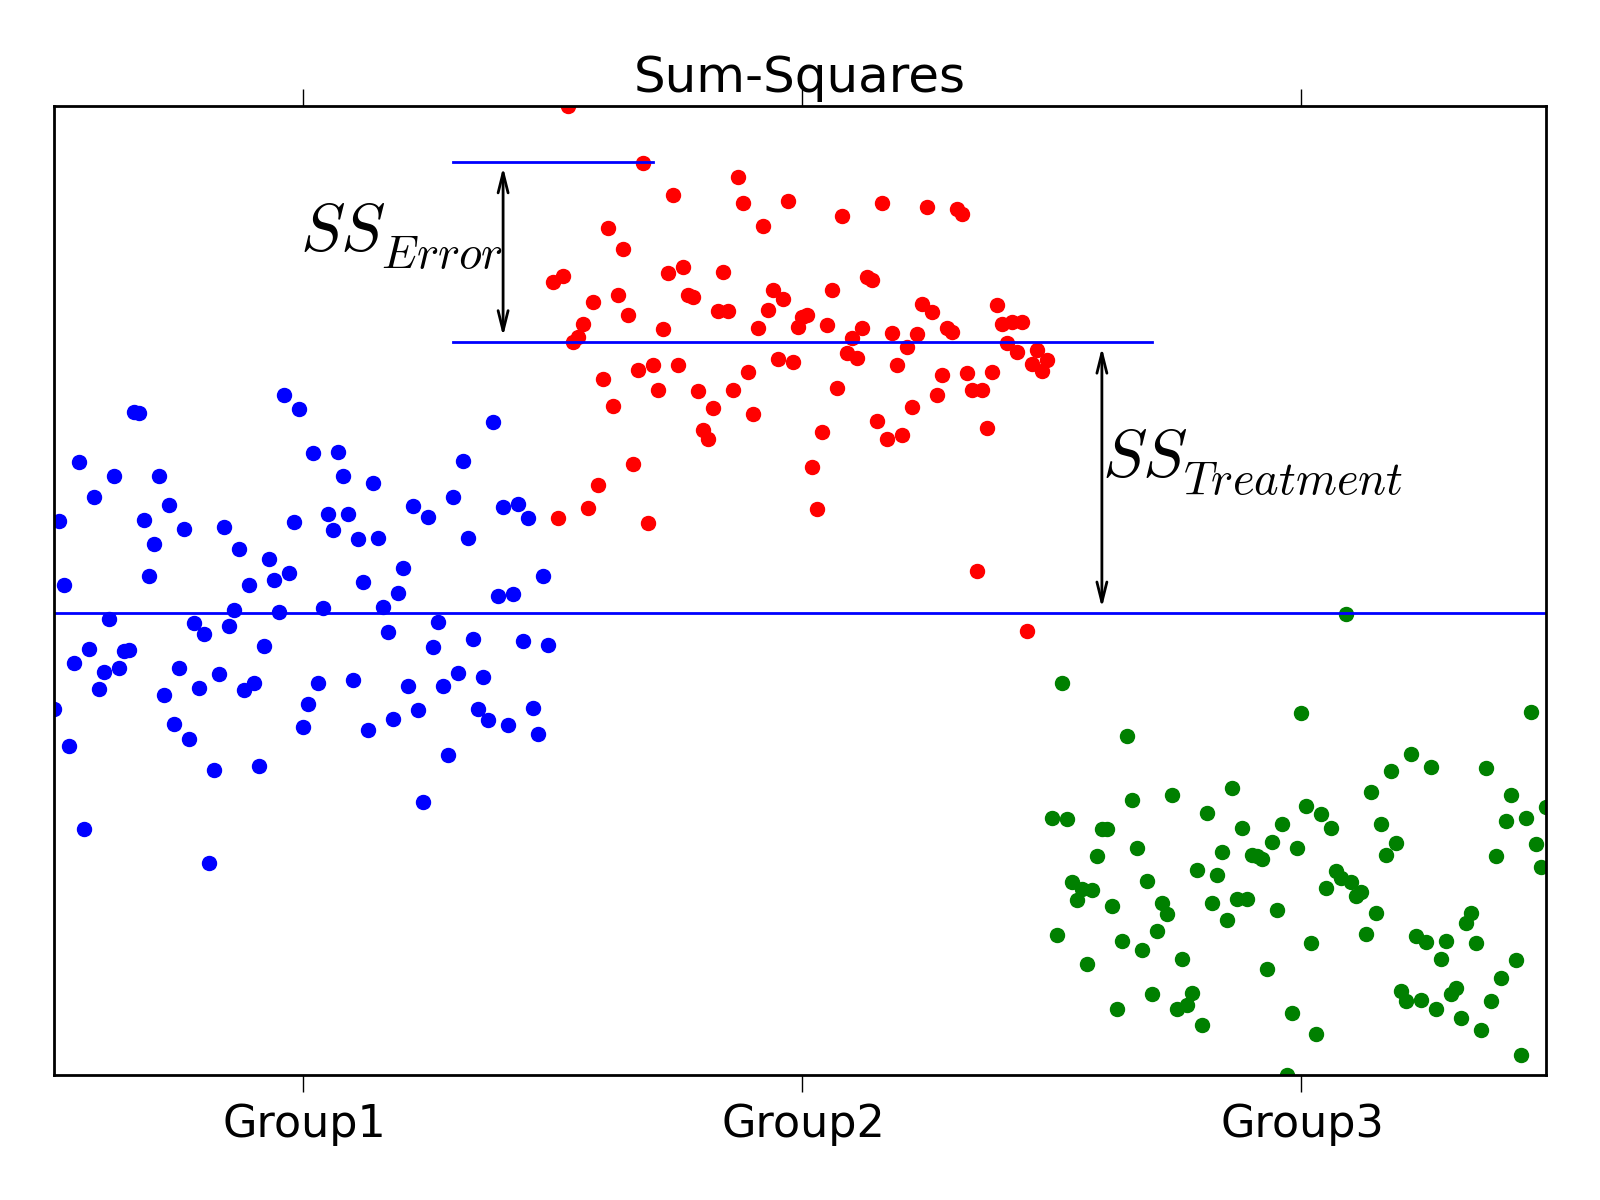
\includegraphics[width=0.5\textwidth]{../Images/anova_annotated.png}\\
  \caption{The long blue line indicates the grand mean over all data. The $SS_{Error}$ describes the variability \emph{within} the groups, and the $SS_{Treamtent}$ (summed over all respective points!) the variability \emph{between} groups.}\label{fig:ANOVA_annotated}
\end{figure}

The number of degrees of freedom DF can be partitioned in a similar way: one of these components (that for error) specifies a chi-squared distribution which describes the associated sum of squares, while the same is true for "treatments" if there is no treatment effect.

\begin{equation}
  DF_\text{Total} = DF_\text{Error} + DF_\text{Treatments}
\end{equation}


\subsubsection{Example: one-way ANOVA}
As an example, take the red cell folate levels ($\mu g/l$) in three groups of cardiac bypass patients given different levels of nitrous oxide ventilation (Amess et al, 1978), described in the \emph{Python} code example below. In total 22 patients were included in the analysis. I first show the result of this ANOVA test, and then explain the steps to get there.

\begin{verbatim}
                DF    SS          MS     F    p(>F)
  C(treatment)   2  15515.76  7757.88  3.71  0.043
  Residual      19  39716.09  2090.32   NaN    NaN
\end{verbatim}

\begin{itemize}
  \item First the "Sums of squares (SS)" are calculated. Here the SS between treatments is 15515.88, and the SS of the residuals is 39716.09 . The total SS is the sum of these two values.
  \item The mean squares (MS) is the SS divided by the corresponding degrees of freedom (DF).
  \item The \emph{F-test}\index{general}{test!F-test} or \emph{variance ratio test}\index{general}{test!variance ratio} is used for comparing the factors of the total deviation. The F-value is the larger mean squares value divided by the smaller value. (If we only have two groups, the F-value is the square of the corresponding t-value. See \ref{py:anovaOneway}).

      \begin{eqnarray}
        F &=& \frac{\text{variance between treatments}}{\text{variance within treatments}} \\
        F &=& \frac{MS_\text{Treatments}}{MS_\text{Error}} = {{SS_\text{Treatments} / (n_{groups}-1)} \over {SS_\text{Error} / (n_{total}-n_{groups})}}
      \end{eqnarray}

  \item Under the null hypothesis that two normally distributed populations have equal variances we expect the ratio of the two sample variances to have an \emph{F Distribution} (see section \ref{sec:ContinuousDistributions}). From the F-value, we can look up the corresponding p-value.
\end{itemize}

\PyImg "anovaOneway.py" (p \pageref{py:anovaOneway}): different aspects of one-way ANOVAs: how to check the assumptions (with the Levene test), different ways to calculate a one-way ANOVA, and a demonstration that for the comparison between groups, a one-way ANOVA is equal to a T-test.
\index{python}{anovaOneway}

\subsection{Multiple Comparisons}\index{general}{Multiple Comparisons}

The Null hypothesis in a one-way ANOVA is that the means of all the samples are the same. So if a one-way ANOVA yields a significant result, we only know that they are \emph{not} the same.

However, often we are not just interested in the joint hypothesis if all samples are the same, but we would also like to know for which pairs of samples the hypothesis of equal values is rejected. In this case we conduct several tests at the same time, one test for each pair of samples. (Typically, this is done with $t-tests$.)

This results, as a consequence, in a \emph{multiple testing problem}:
since we perform multiple comparison tests, we should compensate for the risk of getting a significant result, even if our null hypothesis is true. This can be cone by correcting the p-values to account for this. We have a number of options to do so:

\begin{itemize}
  \item Tukey HSD
  \item Bonferroni correction
  \item Holms correction
  \item ... and others ...
\end{itemize}


\subsubsection{Tukey's Test}\index{general}{test!Tukey's}

\emph{Tukey's test}, sometimes also referred to as the \acrfull{hsd} (HSD) method, controls for the Type I error rate across multiple comparisons and is generally considered an acceptable technique. It is based on a
statistic that we have not come across yet, the \emph{studentized range}\index{general}{studentized range}, which is commonly represented by the variable q. The \emph{studentized range} computed from a list of numbers $x_1, ..., x_n$ is given by

\begin{equation}
  q _{n}= \frac{\max\{\,x_1,\ \dots \ x_n\,\} - \min\{\,x_1,\ \dots\ x_n\}}{s}
\end{equation}

where \emph{s} is the sample standard deviation.
In the Tukey HSD method the sample $x_1, ..., x_n$ is a sample of means and $q$ is the basic test-statistic. It can be used as post-hoc analysis to test between which two groups means there is a significant difference (pairwise comparisons) after rejecting the null hypothesis that all groups are from the same population (i.e. all means are equal).

\PyImg "multipleTesting.py" (p \pageref{py:multipleTesting}): this script provides an example where three treatments are compared.
\index{python}{multipleTesting}

\begin{figure}
  \centering
  \includegraphics[width=0.5\textwidth]{../Images/MultComp.png}\\
  \caption{Comparing the means of multiple groups - here three different treatment options.}
\end{figure}

\subsubsection{Bonferroni correction}\index{general}{Bonferroni correction}

Tukey's studentized range test (HSD) is a test specific to the comparison of all pairs of k independent samples. Instead we can run t-tests on all pairs, calculate the p-values and apply one of the p-value corrections for multiple testing problems. The simplest - and at the same time quite conservative - approach is to divide the required p-value by the number of tests that we do (\emph{Bonferroni correction}). For example, if you perform 4 comparisons, you check for significance not at $p=0.05$, but at $p=0.0125$.

While multiple testing is not yet included in \emph{Python} standardly, you can get a number of multiple-testing corrections done with the statsmodels package:

\begin{lstlisting}
  In[7]: from statsmodels.sandbox.stats.multicomp import multipletests
  In[8]: multipletests([.05, 0.3, 0.01], method='bonferroni')
Out[8]:
  (array([False, False,  True], dtype=bool),
  array([ 0.15,  0.9 ,  0.03]),
  0.016952427508441503,
  0.016666666666666666)
\end{lstlisting}

\subsubsection{Holms correction}\index{general}{Holms correction}

The Holm adjustment sequentially compares the lowest p-value with a Type I error rate that is reduced for each consecutive test. For example, if you have three groups (and thus three comparisons), this means that the first p-value is tested at the .05/3 level (.017), the second at the .05/2 level (.025), and third at the .05/1 level (.05).
As stated by Holm (\cite{Holm1979})"Except in trivial non-interesting cases the sequentially rejective Bonferroni test has strictly larger probability of rejecting false hypotheses and thus it ought to replace the classical Bonferroni test at all instants where the latter usually is applied."

\subsection{Kruskal-Wallis test}\index{general}{test!Kruskal-Wallis}\label{test:Kruskal-Wallis}

When we compare \emph{two} groups to each other, we use the \emph{t-test} when the data are normally distributed and the non-parametric \emph{Mann-Whitney test} otherwise. For \emph{three or more }groups, the test for normally distributed data is the \emph{ANOVA-test}; for not-normally distributed data, the corresponding test is the \emph{Kruskal-Wallis test}. When the null hypothesis is true the test statistic for the Kruskal-Wallis test follows the \emph{Chi squared distribution}.

\PyImg "KruskalWallis.py" (p \pageref{py:KruskalWallis}): Example of a Kruskal-Wallis test (for not normally distributed data).
\index{python}{KruskalWallis}

\section{Exercises}

\subsection*{One or Two Groups}

\begin{enumerate}
  \item \textbf{Paired T-Test} and \textbf{Wilcoxon signed rank sum test}

The daily energy intake from 11 healthy women is [5260., 5470., 5640., 6180., 6390., 6515., 6805., 7515., 7515., 8230., 8770.] kJ.

    Is this value significantly different from the recommended value of 7725?
    (Correct answer: yes, $p_{ttest}=0.018$, and $p_{Wilcoxon}=0.026$)

  \item \textbf{t-test of independent samples}

In a clinic, 15 lazy patients weight [76, 101, 66, 72, 88, 82, 79, 73, 76, 85, 75, 64, 76, 81, 86.] kg, and 15 sporty patients weigh [ 64, 65, 56, 62, 59, 76, 66, 82, 91, 57, 92, 80, 82, 67, 54] kg.

    Are the lazy patients significantly heavier?
    (Correct answer: yes, p=0.045)

  \item \textbf{Normality test}

    Are the two datasets normally distributed?
    (Correct answer: yes, they are)

  \item \textbf{Mann-Whitney test}

    Are the lazy patients still heavier, if you check with the Mann-Whitney test?
    (Correct answer: yes, p=0.039)
\end{enumerate}

\subsection*{Multiple Groups}

(The following example is taken from the really good, but somewhat advanced book by AJ Dobson: "An Introduction to Generalized Linear Models")

\begin{enumerate}
  \item \textbf{Get the data}

    The file   \emph{https://github.com/thomas-haslwanter/statsintro/blob/master/Data/data\_others/Table 6.6 Plant experiment.xls} contains data from an experiment with plants in three different growing conditions. Get the data into \emph{Python}.
    Hint: use the module xlrd

  \item \textbf{Perform an ANOVA}

    Are the three groups different?
    (Correct answer: yes, they are.)

  \item \textbf{Multiple Comparisons}

    Using the Tukey test, which of the pairs are different?
    (Correct answer: only TreamtmentA and TreatmentB differ)

  \item \textbf{Kruskal-Wallis}

    Would a non-parametric comparison lead to a different result?
    (Correct answer: no)

\end{enumerate}
